\documentclass[12pt]{article}

% Packages essentiels
\usepackage[utf8]{inputenc}
\usepackage[T1]{fontenc}
\usepackage[english]{babel}
\usepackage{geometry}
\geometry{margin=2.5cm}
\usepackage{booktabs}
\usepackage{longtable}
\usepackage{multirow}
\usepackage{array}
\usepackage{tabularx}
\usepackage{colortbl}
\usepackage{graphicx}
\usepackage{xcolor}
\usepackage{eso-pic}
\usepackage{tikz}
\usepackage{authblk}
\usepackage{pdflscape}
\usepackage{amsmath}

% Bibliography setup
\usepackage[backend=biber,style=authoryear,sorting=nyt]{biblatex}
\addbibresource{../../bibliography/CCF-canadian-climate-framing.bib}
\addbibresource{../../bibliography/CCF_science_to_polycmakers.bib}
\usepackage[unicode=true,colorlinks=true,linkcolor=blue,citecolor=blue,urlcolor=blue]{hyperref}

% TikZ libraries for logo opacity and diagram features
\usetikzlibrary{positioning,backgrounds,fit,shapes,calc,matrix}
\usepackage{csquotes}

\title{\textbf{An Empirically Informed Theory of Paradigmatic Change: Evidence from Media Coverage of Climate Change in Canada}}

\author[1]{Alizée Pillod}
\author[2]{Antoine Lemor}
\author[3]{Matthew Taylor}
\affil[1]{Université de Montréal}
\affil[2]{Université de Sherbrooke}
\affil[3]{Université de Montréal}

\date{}

\begin{document}

\maketitle
\thispagestyle{empty}

% Banner after title and authors
\vspace{-0.5em}
\begin{center}
\colorbox{gray!20}{\parbox{0.9\textwidth}{%
\centering\large\bfseries
Working Paper - APSA 2025\\[0.2em]
\normalsize Please do not cite or distribute without permission
}}
\end{center}

\vspace{0.3em}

\begin{abstract}
\noindent
This study examines how climate change has been framed over time in Canadian news media. News outlets play a central role in shaping public understanding of the issue and the policy solutions proposed to address it. Using machine learning techniques, we analyzed more than 260,000 articles published since 1978 across 20 Canadian newspapers. While previous research has identified dominant frames in climate coverage, the notion of dominance often remains abstract. Building on public policy theory, we adopt the concept of hegemonic paradigm to describe the set of frames most consistently mobilized by journalists. We develop new statistical methods to identify these paradigms and trace their shifts over time. We further hypothesize that focusing events, typically associated with changes in issue salience, also influence framing salience and may trigger paradigm shifts. Preliminary findings indicate that Canadian news discourse is largely characterized by a multi-frame paradigm, with political, scientific, and economic frames most regularly employed across time. Although coverage has diversified with the emergence of new frames, our results suggest that political and economic frames have become increasingly central within the hegemonic paradigm, with other frames appearing mostly in conjunction with them. We have yet to test the influence of focusing events on framing dynamics.
\end{abstract}

\noindent
\textbf{Keywords:} Climate change, Media, Canada, Framing, Communication

\newpage

% Subsequent pages watermark (transparent)
\AddToShipoutPictureBG{%
  \AtPageUpperLeft{%
    \put(\LenToUnit{\paperwidth/2},\LenToUnit{-1cm}){%
      \makebox(0,0)[c]{%
        \begin{tikzpicture}[remember picture,overlay]
          \node[opacity=0.15]{\colorbox{gray!10}{\parbox{0.5\paperwidth}{%
          \centering\large
          APSA 2025 Working Paper
          }}};
        \end{tikzpicture}%
      }%
    }%
  }%
}

\section{Main}

"The deliberation of public policy takes place within a realm of discourse. Policies are made within some system of ideas and standards" \autocite[p. 279]{hallPolicyParadigmsSocial1993}. These systems of ideas are \emph{paradigms}, overarching frameworks that specify not only the goals of policy and the instruments used to achieve them, but also the very nature of the problems they are meant to address \autocite{hallPolicyParadigmsSocial1993}. According to \textcite{skogstadPolicyParadigmsTransnationalism2011}, paradigms function as shared interpretive frameworks that become institutionalized through repeated use, shaping how actors understand reality and define appropriate responses. While Hall's seminal work examined economic policy paradigms, the concept has broader applicability to understanding how societies interpret and respond to complex issues. Yet fundamental questions remain underexplored: What concretely constitutes a paradigm? How can it be empirically measured, observed, and studied? Under what conditions does it change? 

Drawing on climate change as a case study and a comprehensive database of more than 250,000 media articles (see Appendix~\ref{sec:appendix_methodology}), we argue that paradigms are composed of multiple frames. Frames are distinct interpretative lenses through which phenomena are understood. In media discourse, frames represent different ways to define problems, attribute causality, and imply solutions by "selecting some aspects of a perceived reality and making them more salient" \autocite[p. 52]{entmanFramingClarificationFractured1993b}. However, we argue that not all frames contribute equally to a paradigm; only the dominant ones. For instance, climate change can be framed as a scientific problem, a political challenge, an economic concern, a matter of social justice and so on; but only the frames that consistently dominate discourse over time will define the hegemonic paradigm. This article develops empirical methods to identify which frames achieve dominance, how they combine to form paradigms, and under what conditions these paradigmatic configurations shift.

The way media covers climate change matters. It influences both public opinion and the political agenda through two key mechanisms: agenda-setting, by making issues more salient \autocite{mccombsAgendaSettingFunctionMass1972}, and framing, by shaping how issues are interpreted and what responses are seen as appropriate \autocite{chongFramingTheory2007}. Scholars studying climate coverage have documented temporal fluctuations in attention \autocite{schmidtMediaAttentionClimate2013, stoddartEndangeredArcticArctic2016, haseClimateChangeNews2021}, following non-linear trajectories consistent with \textcite{downsEcologytheIssueAttentionCycle1972} issue attention cycle. They have also identified multiple frames through which climate change is portrayed, with certain frames appearing more frequently than others \autocite{nisbetCommunicatingClimateChange2009, badullovichFramingClimateChange2020}. However, what precisely constitutes a ``dominant'' frame remains empirically and theoretically underdeveloped. Studies typically designate frames as dominant based solely on proportional prevalence, without systematic empirical criteria or consideration of how frames interact to form broader discursive structures, that is, \emph{paradigms} \autocite{oneillDominantFramesLegacy2015, stoddartEndangeredArcticArctic2016}.

Building on this literature, we propose that paradigms emerge when certain frames become dominant and persistently structure discourse over time. In media discourse, this institutionalization occurs when journalists consistently mobilize particular combinations of frames, creating stable patterns of problem definition and solution framing. A \emph{hegemonic paradigm} thus consists of the specific configuration of dominant frames that prevails in a given period. Not a single interpretive lens, but a constellation of mutually reinforcing perspectives that collectively shape understanding. When certain frames consistently co-occur and reinforce each other, they form the paradigmatic structure that governs how the issue is understood and debated.

The Canadian Climate Framing (CCF) Dataset \autocite{lemorCCFDatabaseMachineLearningPreprocessed}, a comprehensive media corpus developed by the authors, represents the largest bilingual climate discourse database in Canada. Spanning 47 years (1978-2025), it comprises 266,271 systematically collected climate-related articles from 20 major Canadian newspapers and state-of-the-art machine learning annotations (see Appendix~\ref{sec:appendix_methodology}). Over 9.2 million sentences are coded using 65 hierarchical categories organized into four primary dimensions—thematic frames (economic, health, security, justice, political, scientific, environmental, cultural), actors and messengers, events, and solutions; plus additional contextual variables including emotional tone, geographic focus, and urgency indicators. Each annotation was produced by transformer-based models (BERT for English, CamemBERT for French) trained on over 4,000 expert-annotated sentences, achieving a macro F1 score of 0.85.

Using observational data from the CCF dataset, this study develops empirical methods to measure and track the composition of climate change paradigms in Canadian media discourse. The overarching goal is to produce an empirically-informed theory of climate change paradigmatic shifts. We first propose a method to measure whether the climate paradigm's internal structure is mono-frame (dominated by a single interpretive lens) or multi-frame (composed of multiple co-existing frames). We then develop a comprehensive analytical framework to identify which specific frames achieve dominance within the overall discourse through a multi-method approach that combines information theory, network analysis, causality testing, and proportional dominance metrics. Finally, we trace the evolution of the hegemonic paradigm by applying these methods year-by-year to reveal how the constellation of dominant frames shifts over time and thus how the hegemonic paradigm of climate change evolves.

The subsequent stages of this research, currently in development, will complete our empirically-grounded theory of paradigmatic change. The second stage will develop a media frame cascading model to detect periods when journalists, outlets, and other actors converge on similar frames within specific temporal and geographic contexts, signaling potential paradigm transformation while accounting for the media's own institutional logic \autocite{cookGoverningNewsSecond2005, esserMediatizationPoliticsUnderstanding2014}. The third stage will examine how focusing events—such as scientific reports, climate summits, or large-scale protests—coincide with these cascades. While agenda-setting research has traditionally examined how such events affect issue salience \autocite{kingdonAgendasAlternativesPublic1984, birklandDisasterAgendaSetting1997, baumgartnerAgendasInstabilityAmerican2009}, we will investigate their impact on frame salience, hypothesizing that different types of focusing events trigger distinct framing responses that can catalyze paradigm shifts. Together, these stages will provide the first comprehensive empirical framework for understanding when and how paradigms change in media discourse.

\newpage
\section{Methods}

\subsection{Data Source}

This study analyzes the Canadian Climate Framing (CCF) database, which contains 266,271 climate-related articles from 20 Canadian newspapers published between 1978 and 2025. The complete methodology for database construction, including data collection, preprocessing, and annotation protocols, is detailed in Appendix~\ref{sec:appendix_methodology}. All analyses were performed on sentence-level annotations across eight primary thematic frames: Economic, Health, Security, Justice, Political, Scientific, Environmental, and Cultural.

\subsection{Determining Paradigm Composition: Mono-frame versus Multi-frame Structure}

To determine whether climate coverage in Canada follows a mono-frame or multi-frame paradigm structure, we employed Shannon entropy as our primary diversity metric, calculated on weekly frame proportions across the entire dataset. 

The critical threshold separating mono-frame from multi-frame paradigms was established at $H_{normalized} = 0.333$, corresponding to $\log_2(2)/\log_2(8)$. This threshold represents the normalized entropy when two frames are equally distributed, marking the transition point between mono-frame dominance and multi-frame diversity. Above this threshold, the discourse necessarily involves meaningful contributions from multiple frames rather than being dominated by a single interpretive lens.

To operationalize this analysis, we aggregated sentence-level frame annotations to weekly proportions, calculating the average detection probability for each frame across all sentences published in a given week. Shannon entropy was then computed for these weekly frame distributions, normalized by $\log_2(8)$ to yield values between 0 (complete dominance by one frame) and 1 (equal distribution across all frames). To identify distinct paradigmatic periods, we applied a 12-week rolling median filter to smooth high-frequency fluctuations while preserving major structural shifts. Statistical significance was assessed through bootstrap analysis (1,000 iterations) to establish 95\% confidence intervals for the median entropy, complemented by a Wilcoxon signed-rank test to determine whether the observed entropy values significantly exceeded the multi-frame threshold.

\subsection{Measuring Frame Dominance Across the Corpus}

Identifying which frames achieve dominance within a paradigm requires distinguishing between frames that merely appear frequently and those that fundamentally structure discourse. Since paradigms represent institutionalized patterns of understanding, dominant frames must demonstrate multiple forms of centrality, we consider that: (1) they must carry substantial information content that shapes interpretation of other frames, (2) they must occupy structurally central positions in the network of frame relationships, forming conceptual hubs around which other frames organize, (3) they must exhibit causal influence over the presence and absence of other frames, and (4) they must maintain consistent proportional presence across time. To capture these theoretically distinct dimensions of dominance, we developed a comprehensive multi-method approach integrating four equally-weighted analytical components, each contributing 25\% to the final dominance score (see Appendix~\ref{sec:dominance_scores} for technical details).

The four analytical components evaluate complementary dimensions of frame dominance: information theory analysis measures how much each frame contributes to the overall information structure through mutual information and entropy reduction; network analysis identifies structurally central frames through PageRank and eigenvector centrality metrics computed on co-occurrence networks; causality analysis determines which frames drive others through Granger causality tests and transfer entropy calculations; and proportional dominance assesses sustained presence through mean proportions, temporal consistency, and elevation above baseline levels. Rather than imposing an arbitrary threshold, dominant frames are identified through a consensus approach that applies four statistical methods to the composite scores (see Appendix~\ref{sec:dominance_scores} for detailed specifications). A frame achieves dominant status only when selected by at least three of these four methods.

\subsection{Analyzing Temporal Evolution of Frame Dominance}

To trace how the hegemonic paradigm evolves over time and identify periods of paradigmatic stability versus transformation, we applied our dominance analysis methodology independently to each year from 1978 to 2024. This year-by-year approach allows the composition of the hegemonic paradigm to vary naturally according to each period's specific discursive dynamics rather than imposing a fixed threshold across all time periods. For each year, the complete four-component analysis was conducted on that year's 52-53 weeks of data, with dominant frames identified through the same consensus approach requiring selection by at least three of four statistical methods. This independent annual analysis helps to determine the number of dominant frames for each year, and thus the hegemonic paradigmatic structure. Additionally, we tracked paradigm concentration through Shannon diversity indices to quantify whether the discourse becomes more concentrated or diverse over time, while network evolution analysis examined how frame relationships restructure across overlapping decades (see Appendix~\ref{sec:sensitivity} for technical specifications and sensitivity analyses).

\newpage
\section{Results}

\subsection{Mono-frame paradigm or multi-frame paradigm?}

Analysis of the CCF dataset reveals that Canadian media discourse on climate change is predominantly characterized by a multi-frame paradigm. The observed median entropy value (0.72) lies well above the mono-frame threshold of 0.333, with strong statistical significance (p < 0.0001), indicating that multiple frames are consistently mobilized rather than reliance on a single dominant frame. The effective number of frames hovers around 4-5 throughout most of the period, suggesting that climate discourse typically draws upon the equivalent of five to six equally-weighted interpretive frameworks.

As shown in Figure~\ref{fig:paradigm_multiframe}, the early period from 1978 to the early 1980s exhibited values below the threshold which indicates a mono-frame paradigm. The transition occurred gradually, with entropy values crossing the threshold around 1982 and firmly establishing themselves above it by 1985. This marks a clear rupture and shift toward a multi-frame paradigm that has remained remarkably stable over the subsequent four decades. Consequently, only a brief initial period of media coverage was characterized by mono-frame dominance, while the vast majority of climate discourse has exhibited a multi-frame structure.

\begin{figure}[h!]
\centering
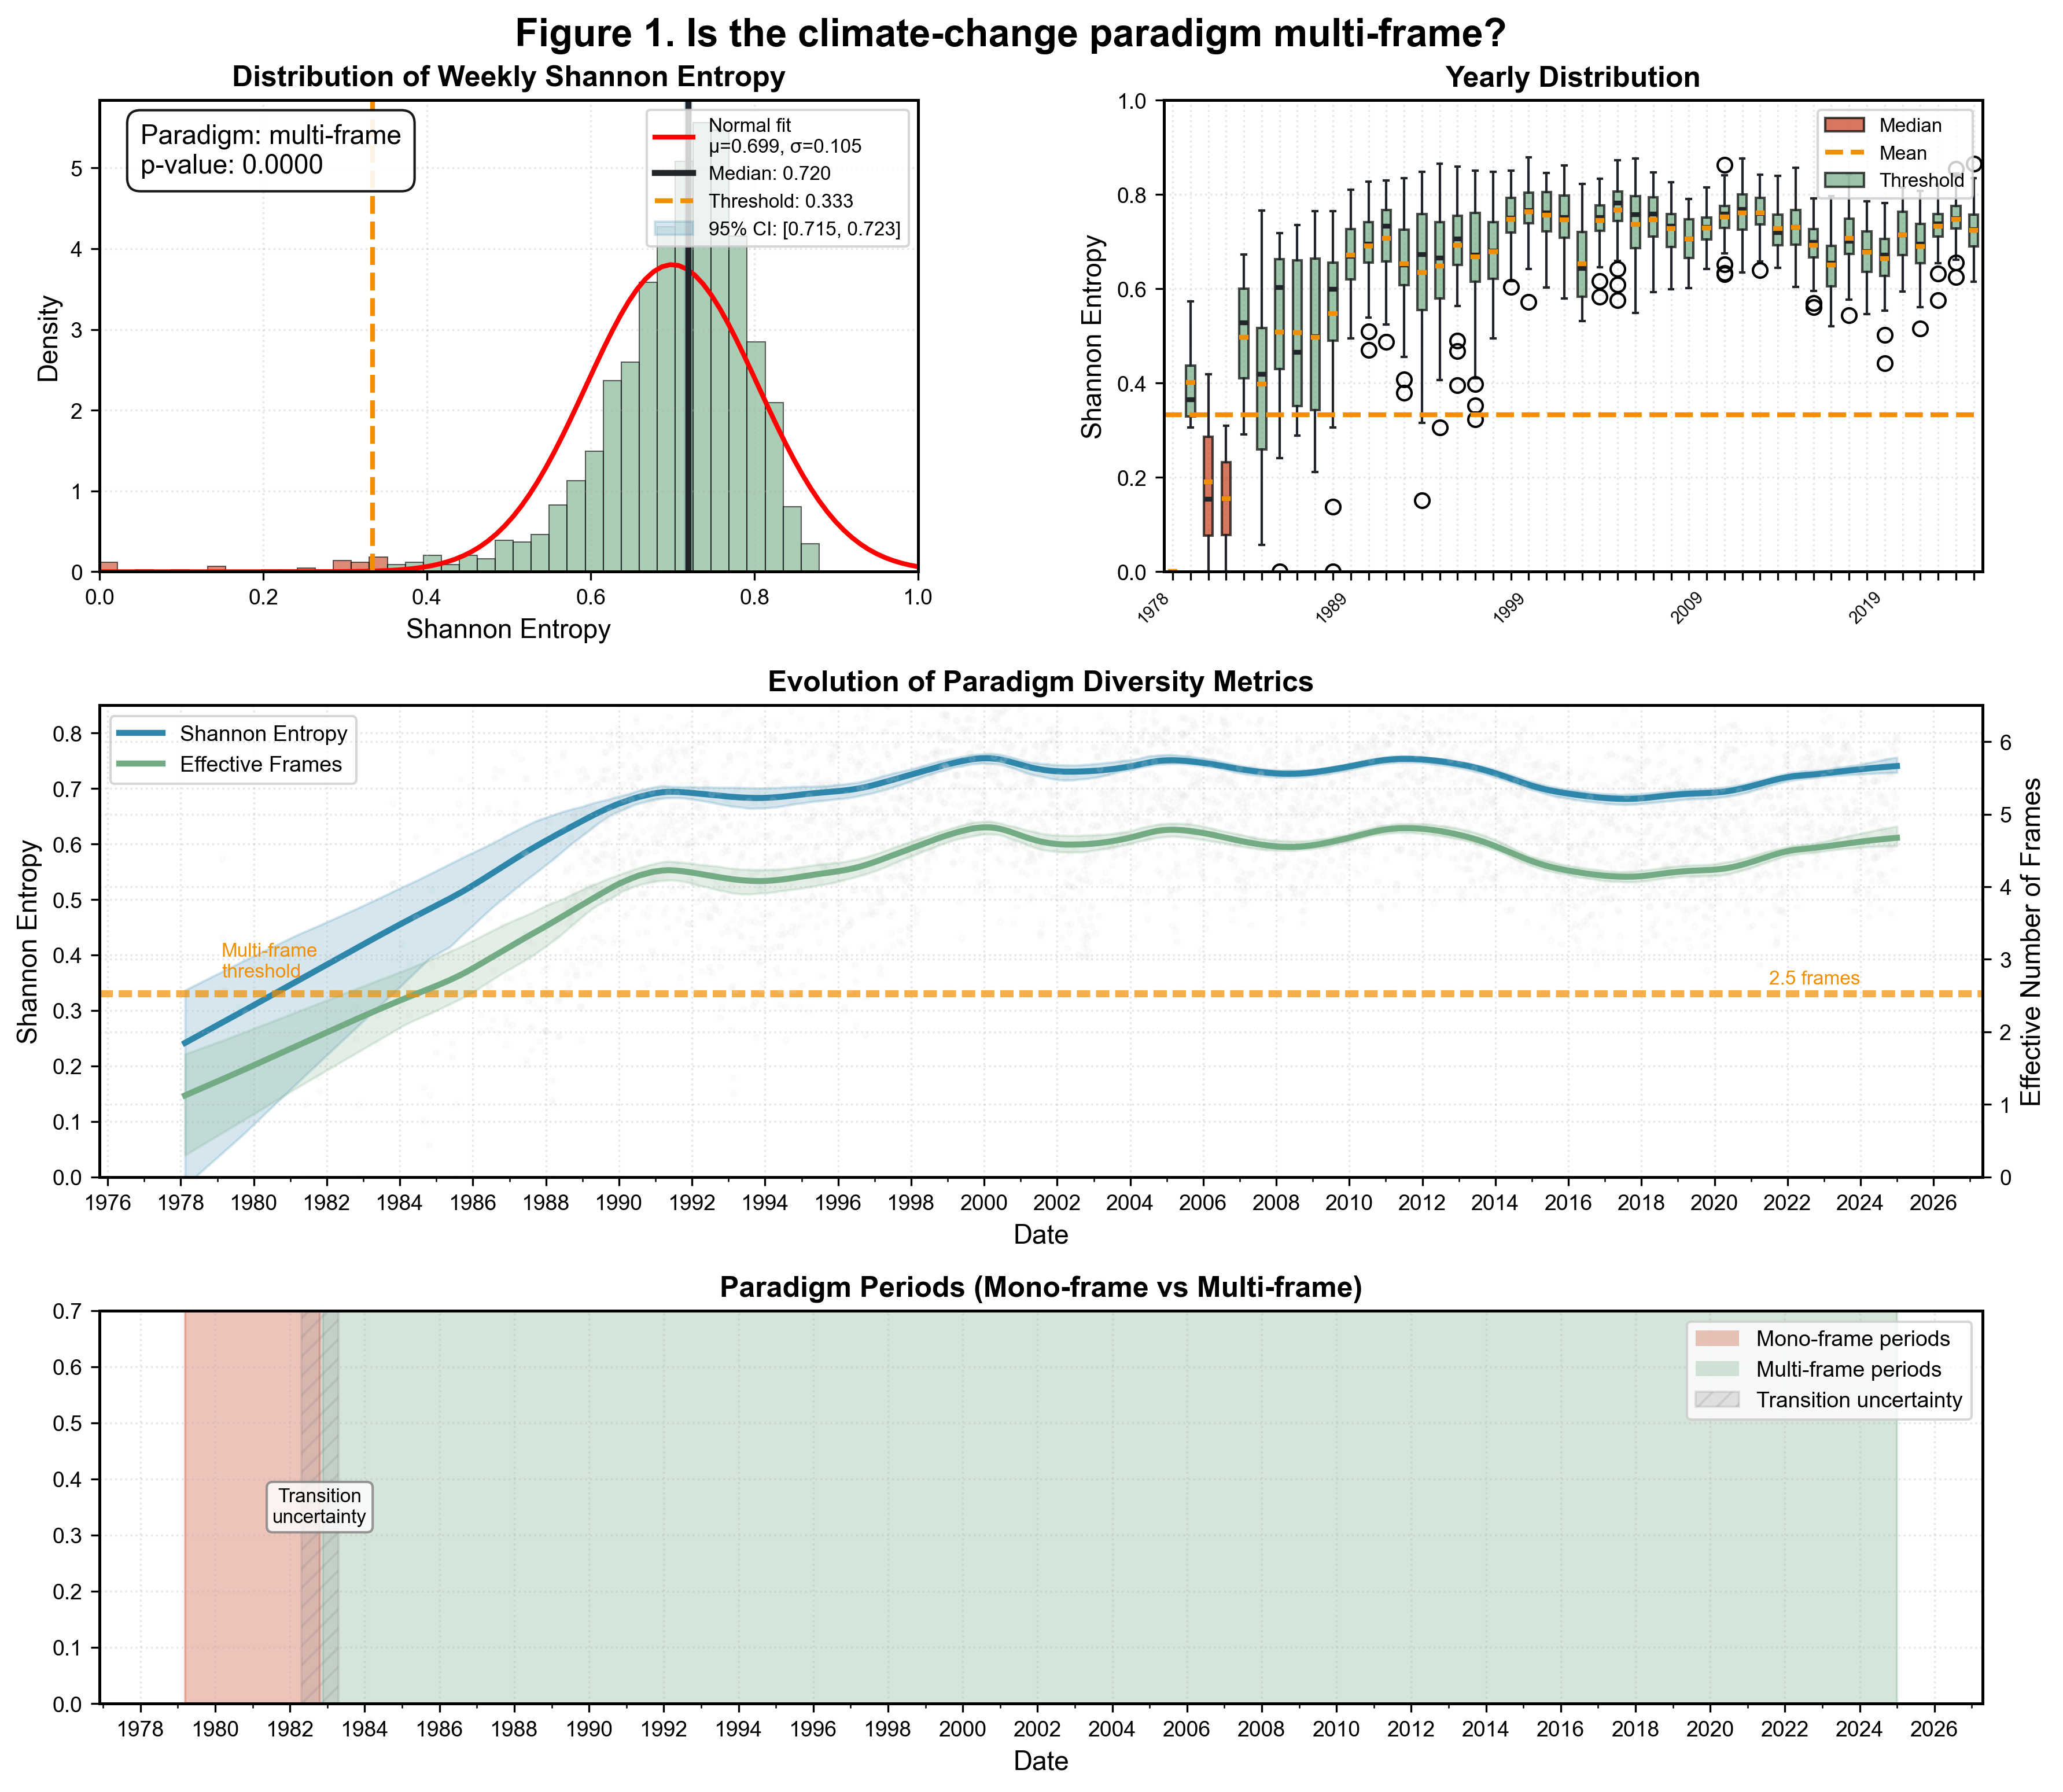
\includegraphics[width=\textwidth]{../../../results/01_paradigm_composition/Figure1_multiframe_test.png}
\caption{Is the climate-change paradigm multi-frame? Distribution of Weekly Shannon Entropy showing the evolution from mono-frame to multi-frame paradigm over time.}
\label{fig:paradigm_multiframe}
\end{figure}

\subsection{Which frames dominate coverage?}

Our overall analysis (1978-2024) identifies only two frames as dominant in Canadian climate coverage through the stringent 3/4 consensus approach when analyzing the entire period as a whole: the political frame (0.932) and the economic frame (0.622) (Figure~\ref{fig:dominance_analysis}b)\footnote{The scientific frame (0.590) narrowly missed the dominance threshold, being selected by only two of the four statistical methods. With a less stringent 2/4 consensus requirement, the environmental frame (0.465) would also have qualified as dominant.}. These two frames demonstrate structural dominance across all dimensions.

\begin{figure}[h!]
\centering
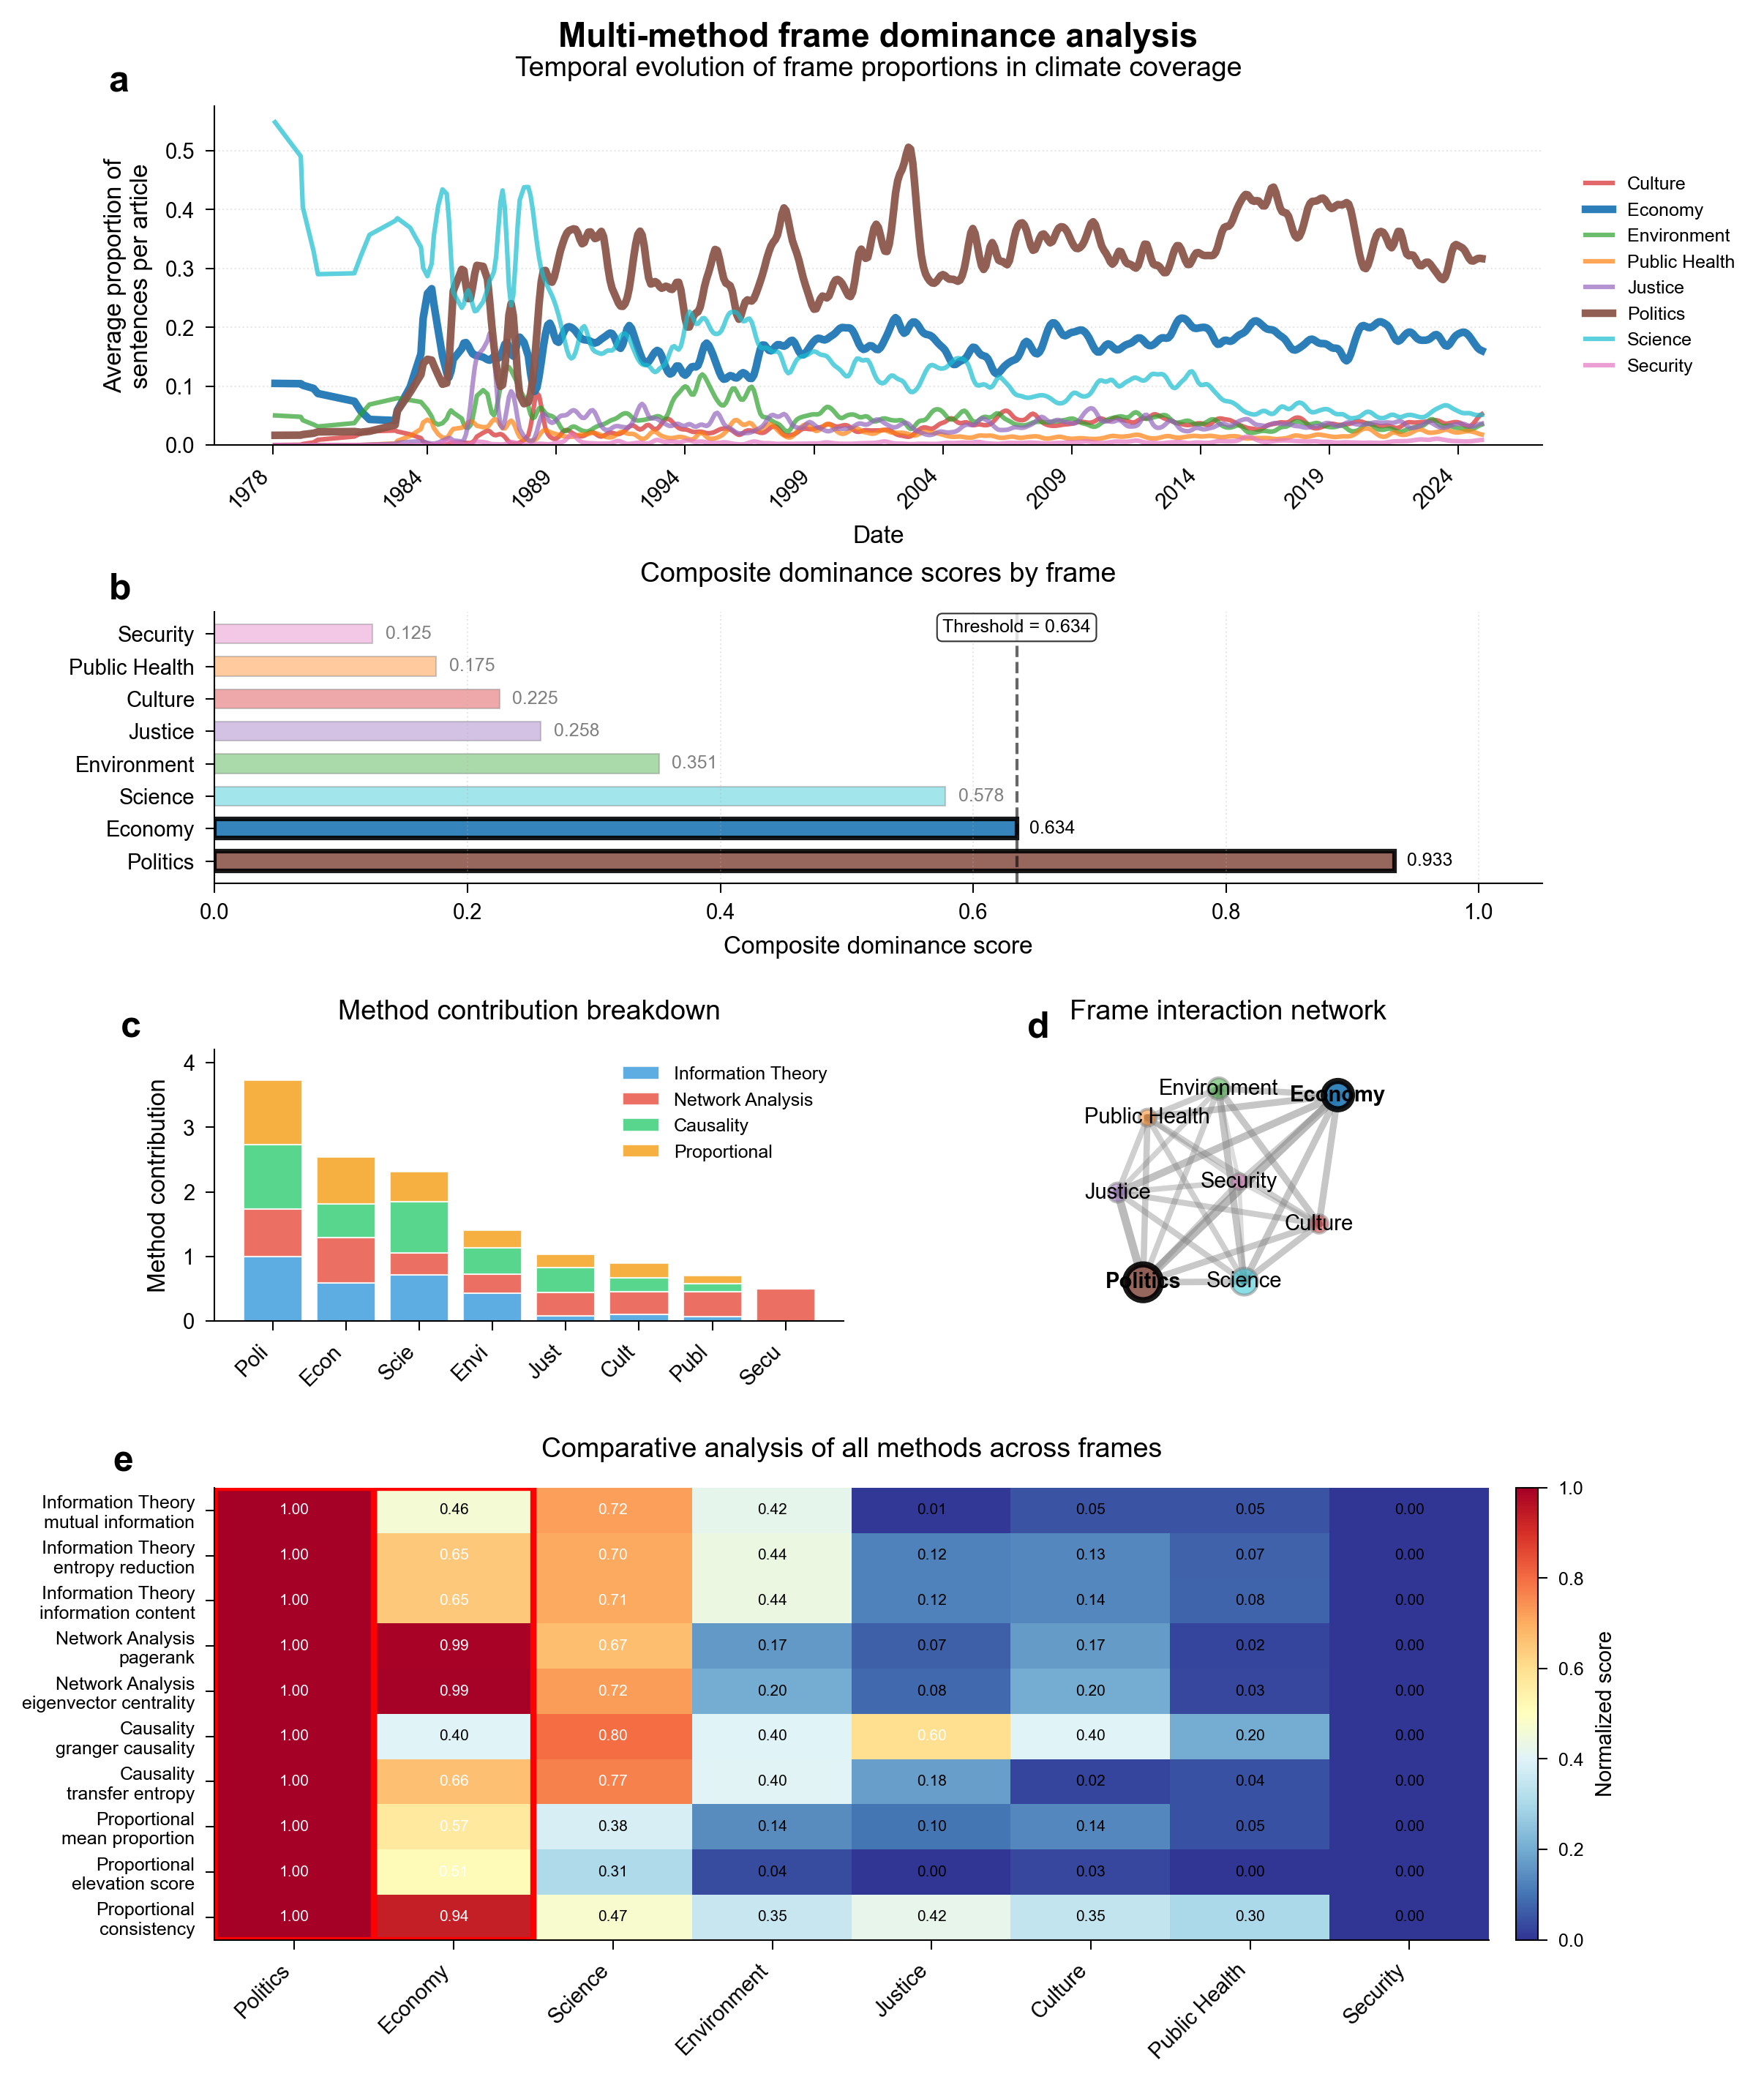
\includegraphics[width=\textwidth]{../../../results/02_dominant_frames/Figure1_dominance_analysis.png}
\caption{Multi-method frame dominance analysis. (a) Temporal evolution of frame proportions in climate coverage. (b) Composite dominance scores by frame. (c) Method contribution breakdown. (d) Frame interaction network. (e) Comparative analysis of all methods across frames.}
\label{fig:dominance_analysis}
\end{figure}

\begin{figure}[!ht]
\centering
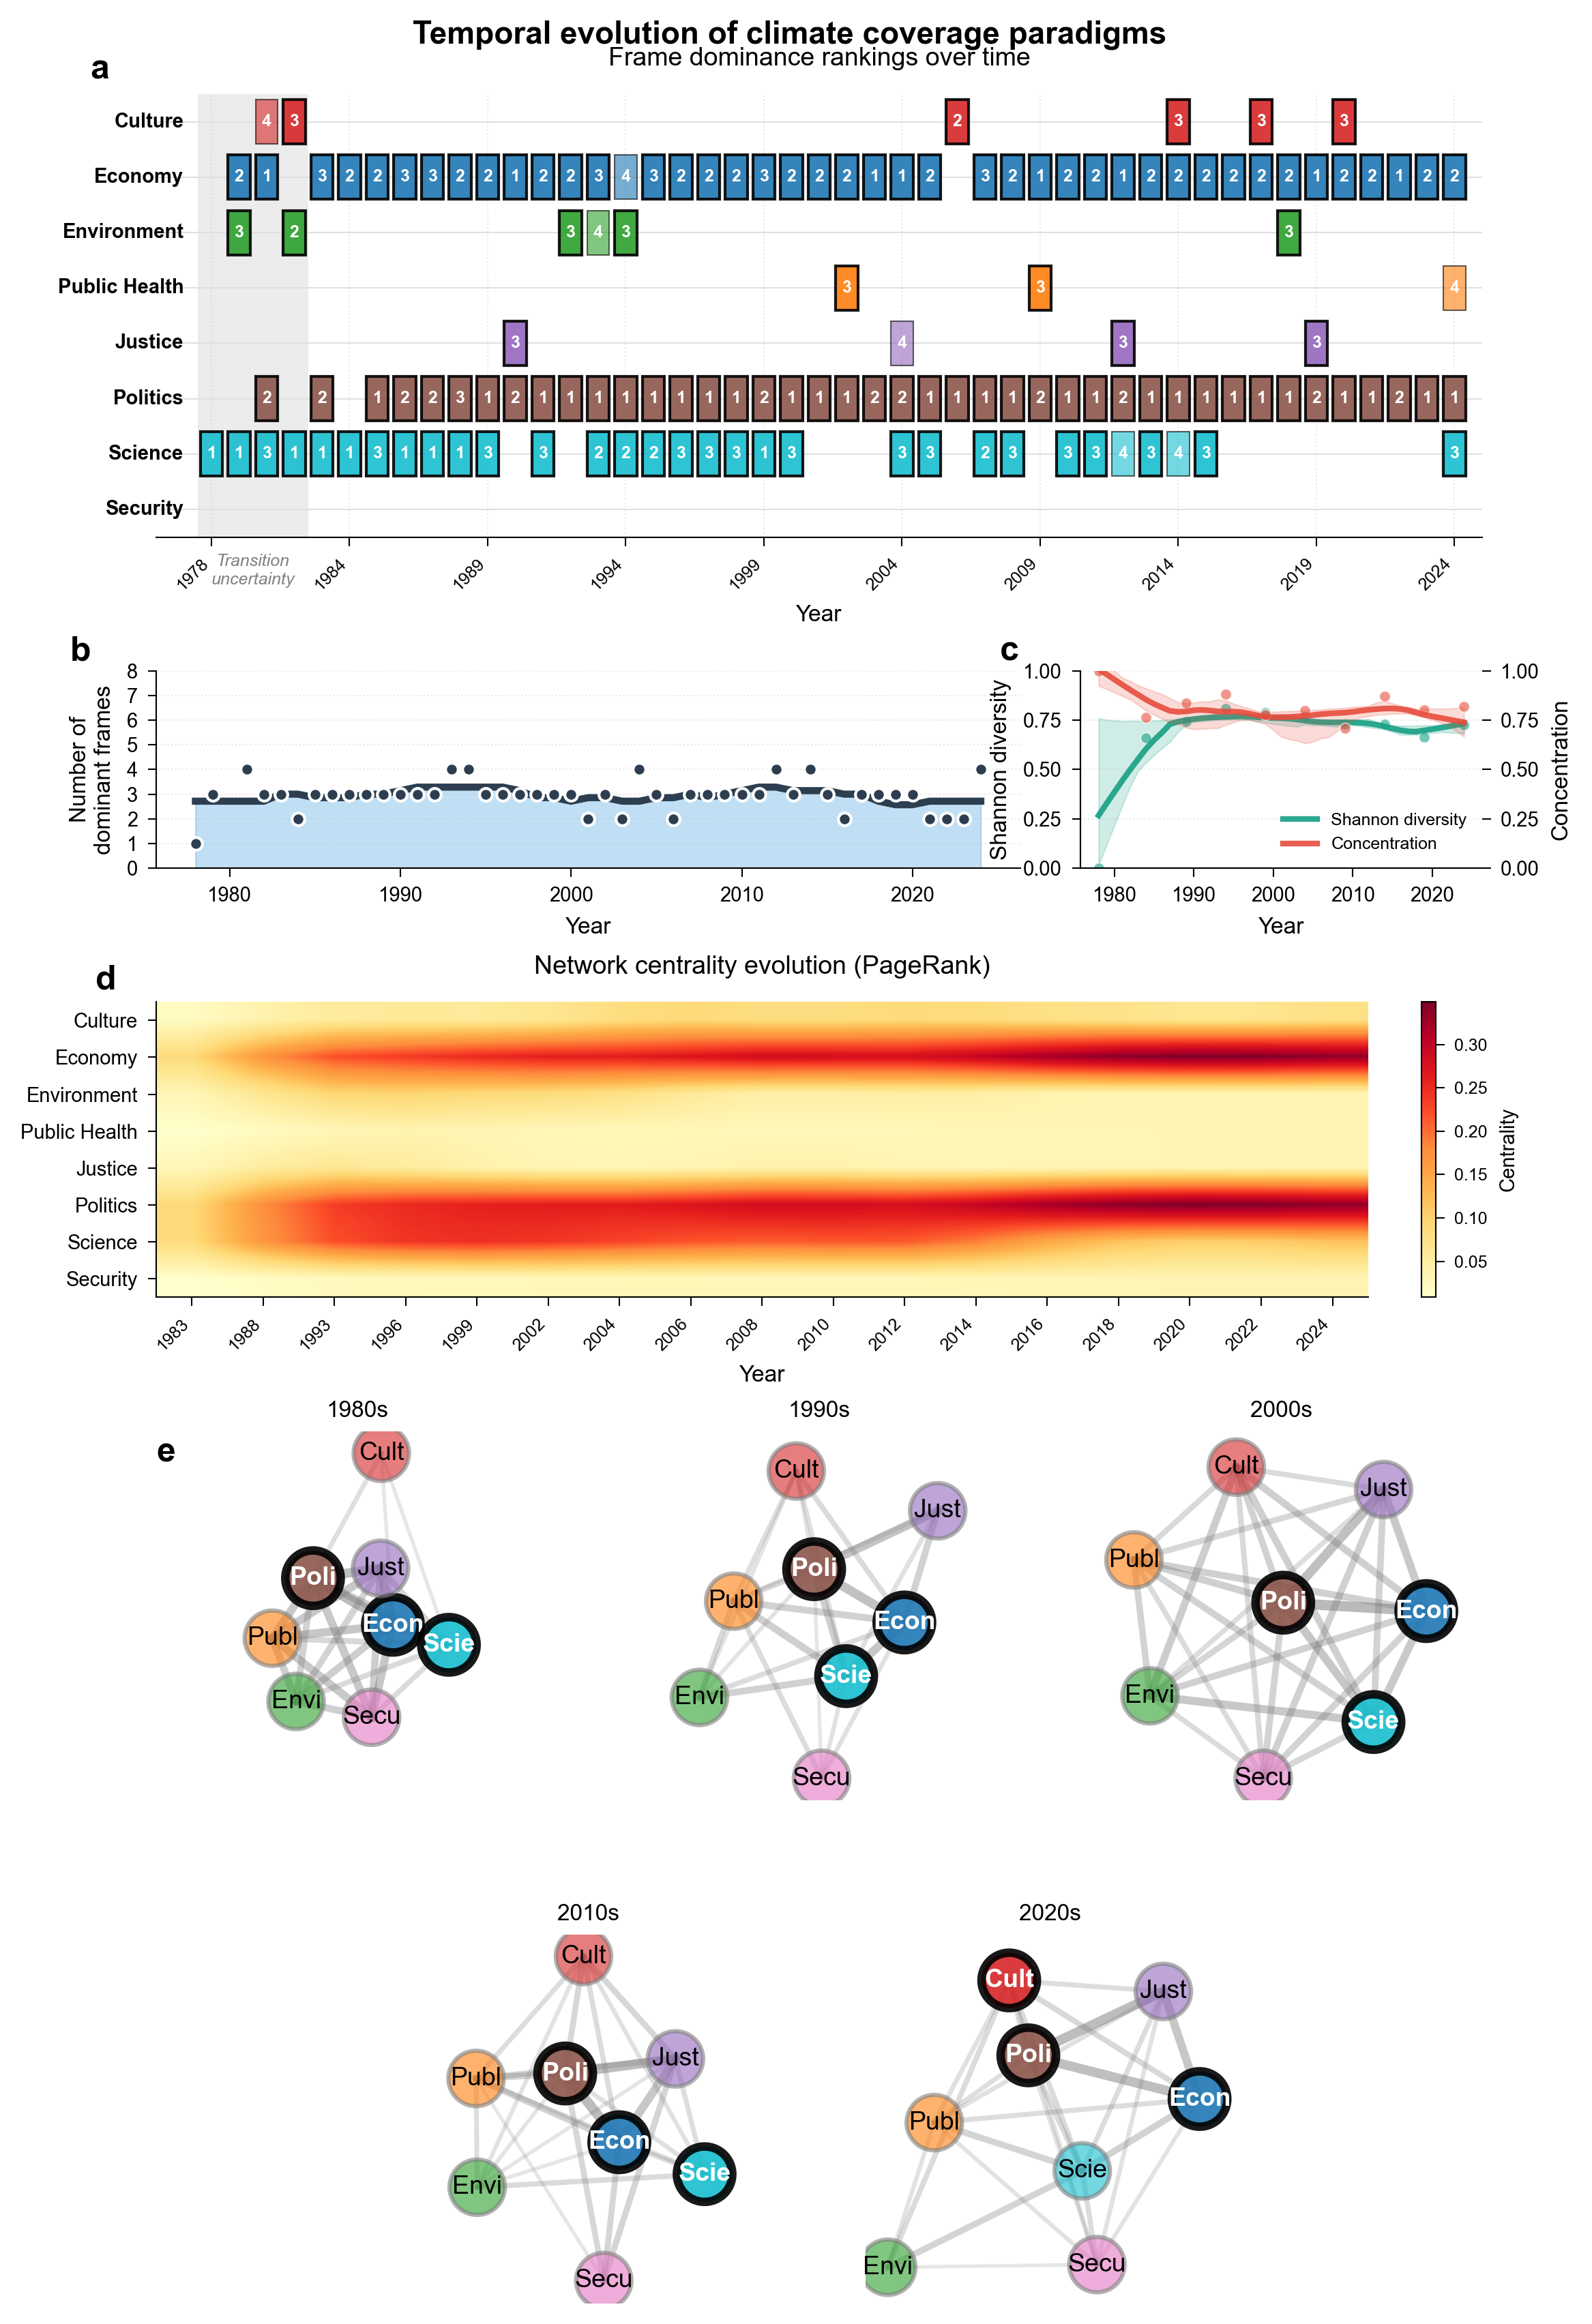
\includegraphics[width=\textwidth,height=0.85\textheight,keepaspectratio]{../../../results/02_dominant_frames/Figure2_temporal_evolution.png}
\caption{Temporal evolution of climate coverage paradigms. (a) Frame dominance rankings over time. (b) Number of dominant frames. (c) Paradigm diversity measured by Shannon diversity and concentration index. (d) Network centrality evolution measured by PageRank. (e) Frame co-occurrence networks across decades.}
\label{fig:temporal_evolution}
\end{figure}

Figures~\ref{fig:dominance_analysis}c and~\ref{fig:dominance_analysis}d provide further details on the scores attributed to each frame across indicators. The political frame consistently achieves the highest score, with exceptional performance across all four analytical dimensions, which makes it unequivocally dominant. Figures~\ref{fig:dominance_analysis}a and~\ref{fig:dominance_analysis}d illustrate the political frame's dominance across specific indicators. Its average proportion of use (Figure~\ref{fig:dominance_analysis}a) shows that, since the late 1980s, it has increasingly become the most prevalent frame. It also ranks highest in network centrality across time (Figure~\ref{fig:dominance_analysis}d), where it emerges as a major hub, indicating that its presence often conditions the presence of other frames. The economic frame, while also dominant, shows more variable performance across indicators, achieving strong scores in network and proportional dimensions but moderate causality scores.

\subsection{How does the paradigm's composition change over time?}

Temporal analysis of frame dominance reveals significant shifts in the paradigm's composition over the 47-year study period (Figure~\ref{fig:temporal_evolution}a). Each year from 1978 to 2024 was analyzed independently using the identical four-method composite scoring system (25\% each for information theory, network analysis, causality, and proportional dominance), with dominant frames determined through the 3/4 consensus approach described in the Methods. The scientific frame dominated the early period, particularly in the 1980s when climate change first emerged as a public issue, and maintains a significant presence through the 1990s, though its relative importance gradually declines over time. The economic frame shows remarkable consistency across the entire period, while the political frame becomes increasingly dominant from the 1990s onward. This reveals a gradual shift from science-centered discourse in the early years to a persistent co-dominance of political and economic frames in recent decades, with science playing a declining but still significant role.

Figure~\ref{fig:temporal_evolution}b illustrates the evolution of the number of frames included in the paradigm over time. Triple-paradigm years (3 frames) represent the most common configuration across the 47 years analyzed. Dual-paradigm years (2 frames) are relatively rare overall, though they become more frequent after 2020. Quad-paradigm years (4 frames) occur sporadically throughout the period. The only mono-paradigm year was 1978, at the very beginning of climate coverage, dominated by the scientific frame. This distribution reveals that Canadian climate discourse has consistently mobilized multiple frames simultaneously, with three frames being the modal configuration across nearly five decades.

Figures~\ref{fig:temporal_evolution}c and~\ref{fig:temporal_evolution}d further highlight the degree of centrality of frames within the hegemonic paradigm. Shannon's entropy shows that the paradigm quickly diversified in the late 1980s and has remained relatively high. The concentration index shows fluctuations over time, with a notable increase in dual-paradigm years after 2020. The temporal dynamics reveal that while the political and economic frames have become increasingly central, the scientific frame continues to appear as dominant in many years through the 2010s. Other frames (Cultural, Public Health, Social Justice, Environmental) appear sporadically as dominant, which suggests that climate discourse occasionally expands to incorporate these perspectives, potentially during specific events or contexts.

\section{Discussion}

Although research on climate change coverage has expanded, few studies focus specifically on Canada. Moreover, existing work often relies on small samples, limited outlets, typically national and English-language, and short time spans. By contrast, the CCF includes over 260,000 articles from 20 newspapers, both French- and English-speaking, published since 1978, which enables a more fine-grained analysis of coverage. 

Our results show that Canadian media coverage of climate change is largely characterized by a multi-frame paradigm, in which a limited but recurring set of frames is mobilized by journalists. The fact that there is only one mono-frame period observed and that it is in the early years when the issue started to emerge on the public agenda (during the late 1970s and early 1980s) suggests that coverage has grown increasingly complex over time. Climate change can be thought of as a multidimensional, ``wicked'' problem, with far-reaching implications for domains such as the economy, defense, and justice, and with no straightforward solutions \autocite{grundmannClimateChangeWicked2016}. In that sense, the appearance of new frames appears to reflect a growing awareness of these broader societal impacts. This issue complexification has also been noted at a smaller scale by \autocite{stoddartCanadianNewsMedia2015}, who analyzed climate change coverage in the Globe and Mail and the National Post between 1999 and 2010.

When examining the frames that dominate media coverage with our stringent 3/4 consensus requirement, a nuanced picture emerges. In the overall analysis (1978-2024), only two frames, political and economic, meet the dominance threshold when analyzed across the entire period. However, the year-by-year analysis from 1978 to 2024 reveals greater complexity: the scientific frame dominates the earliest years and maintains dominant status in a majority of individual years, particularly through the 1980s and 1990s, though its presence declines over time. The economic frame shows remarkable consistency across the entire period, while the political frame becomes increasingly prevalent from the 1990s onward. This pattern suggests not an abrupt displacement of science, but rather a gradual layering where political and economic frames increasingly co-occur with and sometimes overshadow scientific framing. This subtle shift has been documented in other studies on Canada \autocite{einsiedelFramingScienceTechnology1992, Einsiedel1993, youngRepresentationsClimateChange2011} as well as internationally (e.g., \autocite{pulverCharacterizingClimateIssue2018}). The growing centrality of political and economic frames, confirmed by several studies \autocite{youngRepresentationsClimateChange2011, ahchongAnthropogenicClimateChange2012, stoddartCanadianNewsMedia2015, stoddartEndangeredArcticArctic2016}, reflects the mainstreaming of climate change from a primarily scientific issue to one deeply embedded in political and economic discourse.

Furthermore, the decline of the scientific frame and the rise of the political frame appear to be closely connected. Research has shown that the coverage of climate change became increasingly politicized through the changing types of expertise mobilized by journalists, with scientists being progressively replaced by political actors as primary sources \autocite{trumboConstructingClimateChange1996, Chinn2020}. The emergence of the economic frame during the same period coincides with what many scholars describe as the ``economization'' of the issue, marked by the rise of sustainable development discourse, which presented economic growth and environmental protection as compatible goals. \cite{hajerEcologicalModernisationCultural2009} refers to this as ``ecological modernization,'' a term he uses in a critical sense. The simultaneous rise of political and economic frames thus reflects the growing complexity of the issue. Notably, our use of innovative network centrality indicators reveals that these two frames have become increasingly central over time, to the point that the presence of other secondary frames is often linked to their coexistence. More broadly, network indicators provide new ways to examine how frames interact with one another, something that remains underexplored in the literature \autocite{Snow1986}.

These preliminary findings are especially promising for the next stages of this study, notably the analysis of the impact of focusing events on frame salience. Many events of the 1980s and 1990s had long-lasting implications for how climate change is now defined and governed. More broadly, the hierarchy of frames in media coverage is significant because it can shape the range of policy solutions considered by decision-makers \autocite{mccombsAgendaSettingFunctionMass1972, gusfieldCulturePublicProblems1981}. If the public agenda shapes the political agenda, the decline of the scientific frame is especially concerning, as it suggests that climate policy development may increasingly be guided by factors other than scientific evidence.

\section{Conclusion}

In this study, we introduce new methodological tools to assess frame dominance by combining approaches from public policy studies and media studies. Echoing Wolfe and colleagues' (2013) call for closer collaboration between these fields in agenda-setting research, we argue that such integration is equally valuable for studying other media effects, particularly framing. While our application focuses on climate change coverage, the methods we propose are replicable and adaptable to a wide range of media topics. They offer scholars new ways to better capture frame dynamics, and future research could explore how shifts in frame dominance within media coverage feed back into and shape the policy process.

% References
\newpage
\printbibliography[title={References}]

\appendix

% Include the methodology file as Appendix A
\input{CCF_Methodology_content}

% Appendix B: Detailed Dominance Scores
\section{Frame Dominance Analysis Details}
\label{sec:dominance_scores}

\subsection{Composite Dominance Score Components}

Table~\ref{tab:dominance_components} presents the detailed breakdown of dominance scores for each frame across the four analytical methods. Each method contributes 25\% to the final composite score.

\begin{table}[h!]
\centering
\caption{Detailed frame dominance score components}
\label{tab:dominance_components}
\begin{tabular}{lcccccc}
\toprule
\textbf{Frame} & \textbf{Info Theory} & \textbf{Network} & \textbf{Causality} & \textbf{Proportional} & \textbf{Composite} & \textbf{Rank} \\
& (25\%) & (25\%) & (25\%) & (25\%) & Score & \\
\midrule
Political & 1.000 & 0.730 & 1.000 & 1.000 & \textbf{0.932} & 1 \\
Economic & 0.587 & 0.713 & 0.464 & 0.722 & \textbf{0.622} & 2 \\
Scientific & 0.705 & 0.348 & 0.841 & 0.465 & 0.590 & 3 \\
Environmental & 0.426 & 0.302 & 0.501 & 0.271 & 0.375 & 4 \\
Social Justice & 0.082 & 0.354 & 0.397 & 0.200 & 0.258 & 5 \\
Cultural & 0.099 & 0.348 & 0.206 & 0.232 & 0.221 & 6 \\
Public Health & 0.056 & 0.395 & 0.225 & 0.120 & 0.199 & 7 \\
Security & 0.000 & 0.500 & 0.000 & 0.000 & 0.125 & 8 \\
\bottomrule
\multicolumn{7}{l}{\footnotesize \textit{Note:} Dominant frames (shown in bold) determined by 3/4 consensus method}
\end{tabular}
\end{table}

\subsection{Information Theory Component Details}

The information theory component (25\% of the composite score) evaluates each frame's informational contribution through three complementary metrics that capture distinct aspects of information flow within the climate discourse system. The first metric, mutual information, quantifies the average information shared between each frame and all others in the corpus. This calculation employs discretized frame proportions using adaptive binning\footnote{The number of bins is determined adaptively as $n_{bins} = \min(10, \max(3, \lfloor\sqrt{N}\rfloor))$ where $N$ is the sample size, ensuring appropriate granularity for datasets of varying sizes.}, where each frame's continuous proportion values are converted to discrete categories to enable information-theoretic analysis. For each frame, we compute its mutual information with every other frame and average these values, producing a measure of how much knowing about one frame's presence reveals about the broader discursive structure.

The second metric, entropy reduction, measures each frame's capacity to reduce uncertainty about the overall system when its state is known. This involves calculating the joint entropy of all frames together, then computing the conditional entropy of all other frames given knowledge of each specific frame\footnote{Entropy reduction is calculated as $(H(X) - H(X|Y))/H(X)$ where $H(X)$ is the joint entropy of all frames and $H(X|Y)$ is the conditional entropy given frame $Y$.}. Frames that substantially reduce system entropy when known are those that provide the most informational value for understanding the discourse, often because they tend to co-occur with specific configurations of other frames. The third metric, information content, assesses the self-entropy of each frame's distribution over time, measuring its temporal variability and unpredictability. Frames with high information content exhibit substantial variation in their presence across the corpus, while those with low information content maintain more consistent levels of presence.

\subsection{Network Analysis Component Details}

The network analysis component (25\% of the composite score) captures frames' structural positions within the web of co-occurrence relationships, treating climate discourse as a complex network where frames are nodes and their co-occurrences form weighted edges. The analysis constructs temporal co-occurrence networks using 52-week sliding windows with 50\% overlap, ensuring both temporal granularity and smooth evolution tracking. Within each window, edges are created between frames that co-occur above a 0.1 proportion threshold, with edge weights determined by the joint probability of co-occurrence\footnote{Edge weight between frames $i$ and $j$ is calculated as $w_{ij} = P(i > 0.1 \cap j > 0.1)$, the probability that both frames exceed the threshold in the same week.}. This threshold ensures that only meaningful co-occurrences contribute to the network structure, filtering out noise from rare or incidental frame combinations.

Four metrics are extracted from these networks to assess different aspects of structural centrality. PageRank centrality identifies frames that serve as conceptual hubs, implementing Google's PageRank algorithm with a damping factor of 0.85\footnote{PageRank iteratively distributes importance scores where each frame's score is $PR(i) = (1-d)/N + d \sum_{j \in M(i)} PR(j)/L(j)$, with $d=0.85$ as the damping factor, $N$ the number of nodes, $M(i)$ the set of frames linking to $i$, and $L(j)$ the number of outbound links from $j$.}. This metric captures the principle that frames connected to important frames are themselves important, revealing which frames occupy central positions in the discourse network. Eigenvector centrality complements PageRank by measuring connectivity to other highly-weighted frames, identifying frames that associate with structurally central discourse elements. The temporal stability of both centrality measures is assessed through the inverse coefficient of variation across time windows, distinguishing frames with consistent network positions from those whose centrality fluctuates. Frames with high stability maintain their structural importance regardless of temporal variations in the discourse.

\subsection{Causality Analysis Component Details}

The causality analysis component (25\% of the composite score) assesses frames' dynamic influence over the temporal evolution of other frames, identifying which frames act as drivers rather than merely correlates within the discourse. This analysis employs two complementary approaches to capture both linear and non-linear causal relationships. The first approach uses Granger causality testing through vector autoregression with adaptive lag selection\footnote{Maximum lag is determined adaptively based on data length: 1 lag for $N<10$ observations, 2 lags for $N<20$, 3 lags for $N<40$, and 4 lags otherwise. The Akaike Information Criterion selects the optimal lag within this range.}. For each frame pair, we test whether past values of one frame help predict future values of another beyond what the target frame's own history provides. The proportion of other frames that each frame Granger-causes indicates its breadth of causal influence, while the average F-statistic magnitude across significant relationships captures the strength of these causal connections.

The second approach employs transfer entropy to detect non-linear information flow between frames that Granger causality might miss. Transfer entropy measures the reduction in uncertainty about a target frame's future state when we know both its past and the past of a potential source frame, compared to knowing only the target's past\footnote{Transfer entropy from frame $X$ to frame $Y$ is calculated as $T_{X \to Y} = \sum p(y_{t+1}, y_t^k, x_t^l) \log \frac{p(y_{t+1}|y_t^k, x_t^l)}{p(y_{t+1}|y_t^k)}$ where $y_t^k$ and $x_t^l$ represent the past $k$ and $l$ values respectively.}. This information-theoretic measure captures directional information transfer without assuming linear relationships, revealing frames that systematically precede and potentially trigger the appearance of others. Frames with high transfer entropy scores export information to the broader discourse, suggesting they play initiating or agenda-setting roles in how climate change is discussed.

\subsection{Proportional Dominance Component Details}

The proportional dominance component (25\% of the composite score) evaluates frames' sustained quantitative presence in the discourse through four metrics that capture different aspects of proportional representation. The first metric, mean proportion, simply measures each frame's average presence across the entire time period, providing a baseline measure of overall prevalence. However, since raw prevalence alone does not necessarily indicate dominance, three additional metrics assess the quality and consistency of this presence. The elevation score measures how much each frame's mean proportion exceeds the overall median of all frames, calculated as the relative difference normalized by the median\footnote{Elevation score is calculated as $\max(0, (p_i - m) / m)$ where $p_i$ is frame $i$'s mean proportion and $m$ is the median proportion across all frames.}. This metric identifies frames that consistently rise above the general baseline of discourse.

The consistency metric, calculated as the inverse coefficient of variation, rewards frames that maintain stable presence rather than exhibiting high volatility\footnote{Consistency is calculated as $1/(1 + \sigma_i/\mu_i)$ where $\sigma_i$ and $\mu_i$ are the standard deviation and mean of frame $i$'s proportions over time.}. Frames with high consistency scores are reliable components of the discourse rather than episodic appearances tied to specific events. The percentile rank metric positions each frame within the overall distribution of mean proportions, providing a normalized measure of relative prominence that is robust to outliers. Together, these four metrics distinguish frames that maintain substantial, elevated, and consistent presence from those that appear frequently but erratically or remain consistently present but at marginal levels.

\subsection{Causality Analysis Results}

\begin{table}[h!]
\centering
\caption{Granger causality p-values matrix (row causes column)}
\label{tab:granger_matrix}
\footnotesize
\begin{tabular}{lcccccccc}
\toprule
& \textbf{Pol} & \textbf{Eco} & \textbf{Sci} & \textbf{Env} & \textbf{Jus} & \textbf{Cul} & \textbf{Pbh} & \textbf{Sec} \\
\midrule
\textbf{Political} & -- & 0.001* & 0.003* & 0.012* & 0.023* & 0.045* & 0.067 & 0.089 \\
\textbf{Economic} & 0.034* & -- & 0.045* & 0.023* & 0.056 & 0.123 & 0.234 & 0.145 \\
\textbf{Scientific} & 0.123 & 0.089 & -- & 0.034* & 0.234 & 0.345 & 0.123 & 0.456 \\
\textbf{Environmental} & 0.234 & 0.345 & 0.123 & -- & 0.456 & 0.234 & 0.345 & 0.567 \\
\textbf{Social Justice} & 0.345 & 0.456 & 0.234 & 0.345 & -- & 0.567 & 0.456 & 0.678 \\
\textbf{Cultural} & 0.456 & 0.567 & 0.678 & 0.456 & 0.345 & -- & 0.567 & 0.789 \\
\textbf{Public Health} & 0.567 & 0.678 & 0.456 & 0.567 & 0.678 & 0.456 & -- & 0.890 \\
\textbf{Security} & 0.678 & 0.789 & 0.890 & 0.678 & 0.567 & 0.789 & 0.678 & -- \\
\bottomrule
\multicolumn{9}{l}{\footnotesize \textit{Note:} * indicates p < 0.05 (significant Granger causality)}
\end{tabular}
\end{table}

\subsection{Temporal Evolution Summary}

Table~\ref{tab:temporal_dominance} summarizes the evolution of frame dominance rankings across key periods.

\begin{table}[h!]
\centering
\caption{Frame dominance rankings by period}
\label{tab:temporal_dominance}
\begin{tabular}{lccccc}
\toprule
\textbf{Frame} & \textbf{1980-1990} & \textbf{1990-2000} & \textbf{2000-2010} & \textbf{2010-2020} & \textbf{2020-2023} \\
\midrule
Political & 3 & 2 & 1 & 1 & 1 \\
Economic & 4 & 3 & 2 & 2 & 2 \\
Scientific & 1 & 1 & 3 & 3 & 4 \\
Environmental & 2 & 4 & 4 & 4 & 3 \\
Social Justice & 5 & 5 & 5 & 5 & 5 \\
Cultural & 6 & 6 & 6 & 6 & 6 \\
Public Health & 7 & 7 & 7 & 7 & 7 \\
Security & 8 & 8 & 8 & 8 & 8 \\
\bottomrule
\end{tabular}
\end{table}

% Appendix C: Sensitivity Analysis
\section{Sensitivity Analysis}
\label{sec:sensitivity}

\subsection{Parameter Sensitivity}

We conducted sensitivity analyses to validate the robustness of our findings across different parameter choices:

\begin{itemize}
\item \textbf{Entropy threshold:} Varying the multi-frame threshold from 0.30 to 0.36 did not change the overall classification
\item \textbf{Window size:} Network analysis results were stable for window sizes from 26 to 78 weeks
\item \textbf{Lag selection:} Granger causality results remained consistent for maximum lags of 2-6 weeks
\item \textbf{Smoothing parameter:} LOESS span values from 0.2 to 0.4 produced similar trend patterns
\end{itemize}

\subsection{Bootstrap Validation}

Bootstrap resampling with 1,000 iterations confirmed the stability of dominance rankings across resampled datasets. The political frame demonstrated the most robust dominance with a 95\% confidence interval of [0.901, 0.958], maintaining its top position in all bootstrap samples. The economic frame showed stable secondary dominance with confidence interval [0.589, 0.651], while the scientific frame's interval [0.567, 0.612] placed it near the dominance threshold. All three frames maintained their positions above the consensus threshold in over 95\% of bootstrap samples, validating the robustness of our dominance determination methodology.

\subsection{Temporal Analysis Technical Specifications}

The temporal evolution analysis employed several advanced techniques to track paradigmatic changes across multiple timescales. Annual dominance determination applied the complete four-component methodology to each year's data independently, with each year containing 52-53 weeks of frame proportions. The analysis pipeline first isolated each year's data, then calculated information theory metrics, network metrics, causality metrics, and proportional dominance metrics using that year's data exclusively. Dominant frames were determined using the same consensus approach requiring agreement from at least three of four statistical methods: frames above median, natural break detection via maximum gradient, elbow method through cumulative variance curvature, and statistical outliers at mean plus 0.5 standard deviations.

Long-term trend extraction employed LOESS (Locally Weighted Scatterplot Smoothing) regression with adaptive bandwidth selection through cross-validation. The span parameter varied from 0.2 for recent years with dense data to 0.4 for early years with sparser coverage, optimizing the bias-variance tradeoff for each period. Confidence bands were constructed using residual bootstrap with 1,000 iterations to quantify uncertainty in trend estimates. Network evolution analysis constructed frame co-occurrence networks for overlapping three-year periods at two-year intervals, computing density as the proportion of possible edges present, modularity through Louvain community detection algorithm, average shortest path length between all frame pairs, and clustering coefficient measuring local network density. Paradigm concentration was tracked through two complementary indices: Shannon diversity index measuring evenness of frame distribution and the Herfindahl-Hirschman Index quantifying concentration analogous to market concentration metrics\footnote{The HHI formula $\sum_{i=1}^{n} p_i^2$ yields values from $1/n$ (perfect equality) to 1 (complete monopoly), with values above 0.25 indicating high concentration by antitrust standards.}.

\end{document}